\documentclass{article}
\usepackage{tabularx}
\usepackage{setspace}
\usepackage{graphicx}
\usepackage{caption}
\usepackage{amsmath}
\usepackage{xcolor}
\usepackage{amssymb}
\usepackage[margin=1in]{geometry}
\usepackage{tikz}
\usetikzlibrary{automata}
\usetikzlibrary{positioning}
\usetikzlibrary{arrows}
\tikzset{	node distance=2.5cm, 
	every state/.style={ 
		semithick,
		fill=gray!10},
	initial text={},     
	double distance=2pt, 
	every edge/.style={  
		draw,
		->, %>=stealth’,     
		auto,
		semithick}
}
\let\epsilon\varepsilon
\usepackage{xepersian}
\settextfont{Yas}
% Fixture for Xepersian 23 bug of setting persian math digit fonts
\ExplSyntaxOn \cs_set_eq:NN \etex_iffontchar:D \tex_iffontchar:D \ExplSyntaxOff
\setmathdigitfont{Yas}
\onehalfspacing
\renewcommand{\labelenumii}{\alph{enumii})}

\begin{document}
	\begin{center}
		\Huge
		مبانی نظریه محاسبه
	\end{center}
	\Large
	\begin{tabularx}{\linewidth}{>{\raggedleft\arraybackslash}X>{\raggedright\arraybackslash}X}
		پاسخ کوییز  دوم
		&
		نمره کل: 25
	\end{tabularx}
	\rule{\textwidth}{1pt}
	\large
	\begin{enumerate}
		\item 
		
		\textcolor{cyan}{
			(7 نمره)
		}
		
		\begin{minipage}{0.5\textwidth}
			\begin{tabularx}{\linewidth}{|c|X|}
				\hline
				$q_0$ &					
پذیرش $\Lambda$ 
				\\ \hline
				$q_1$ &					
رشته با صفر شروع شده و به صفر ختم شده پس تعداد $ \tt 01 $ها با $\tt 10 $ها برابر است.
				\\ \hline
				$q_2$ &			
رشته با صفر شروع شده و به یک ختم شده پس تعداد $ \tt 01 $ها یکی بیشتر از $\tt 10 $ها است.
				\\ \hline
				$q_3$ &				
رشته با یک شروع شده و به یک ختم شده پس تعداد $ \tt 01 $ها با $\tt 10 $ها برابر است.
				\\ \hline
				$q_4$ &					
رشته با یک شروع شده و به صفر ختم شده پس تعداد $\tt 10 $ها یکی بیشتر از $ \tt 01 $ها است.
				\\ \hline
			\end{tabularx}
		\end{minipage}
		\begin{minipage}{0.5\textwidth}
			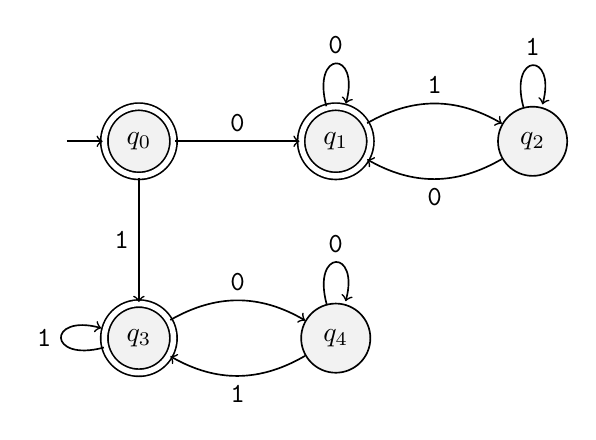
\begin{tikzpicture}
				\node[state, accepting, initial] (q0) {$q_0$};
				\node[state, accepting, right of=q0] (q1) {$q_1$};
				\node[state,  right of=q1] (q2) {$q_2$};
				\node[state, , accepting, below of=q0] (q3) {$q_3$};
				\node[state,  right of=q3] (q4) {$q_4$};
				\draw (q1) edge[loop above] node {\tt 0} (q1);
				\draw (q2) edge[loop above] node {\tt 1} (q2);
				\draw (q3) edge[loop left] node {\tt 1} (q3);
				\draw (q4) edge[loop above] node {\tt 0} (q4);
				\draw (q0) edge node {\tt 0} (q1);
				\draw (q1) edge[bend left] node {\tt 1} (q2);
				\draw (q0) edge node [left] {\tt 1} (q3);
				\draw (q3) edge[bend left] node {\tt 0} (q4);
				\draw (q2) edge[bend left] node {\tt 0} (q1);
				\draw (q4) edge[bend left] node {\tt 1} (q3);
			\end{tikzpicture}
		\end{minipage}
		\begin{center}
			\textcolor{cyan}{
				(۵ نمره)
			}
		\end{center}

		\begin{align*}
			&q_0 101 \longrightarrow 1q_3 01 \longrightarrow 10 q_4 1 \longrightarrow 101q_3 && \text{\textcolor{cyan}{(۱ نمره)}} \\
			&q_0 10010 \longrightarrow 1q_3 0010 \longrightarrow 10 q_4 010 \longrightarrow 100 q_4 10 \longrightarrow 1001 q_3 0 \longrightarrow 10010 q_4 && \text{\textcolor{cyan}{(۱ نمره)}}
		\end{align*}

		\item 
		
		\textcolor{cyan}{
			(4 نمره)
		}
		
		\begin{minipage}{0.5\textwidth}
			\begin{tabularx}{\linewidth}{|c|X|}
				\hline
				$q_0$ &		
رشته به یک ختم شده است و تاکنون مجاور هر صفری، صفر قرار دارد.
				\\ \hline
				$q_1$ &			
رشته به دقیقا ۱ صفر ختم شده است و تاکنون مجاور هر صفری، صفر قرار دارد.
				\\ \hline
				$q_2$ &		
رشته به حداقل ۲ صفر ختم شده است و تاکنون مجاور هر صفری، صفر قرار دارد.
				\\ \hline
				$q_3$ &				
صفری در رشته وجود دارد که هیچ صفری مجاور آن نیست.
				\\ \hline
			\end{tabularx}
		\end{minipage}
		\begin{minipage}{0.5\textwidth}
			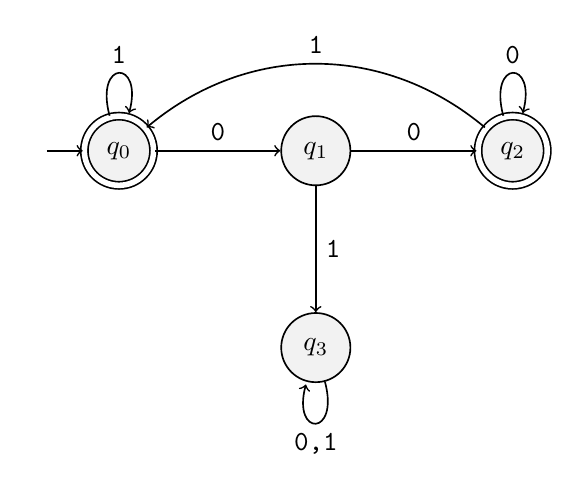
\begin{tikzpicture}
				\node[state, accepting,initial] (q0) {$q_0$};
				\node[state, right of=q0] (q1) {$q_1$};
				\node[state,  accepting, right of=q1] (q2) {$q_2$};
				\node[state, below of=q1] (q3) {$q_3$};
				\draw (q0) edge node {\tt 0} (q1);
				\draw (q1) edge node {\tt 0} (q2);
				\draw (q1) edge node {\tt 1} (q3);
				\draw (q0) edge[loop above] node {\tt 1} (q0);
				\draw (q2) edge[loop above] node {\tt 0} (q2);
				\draw (q3) edge[loop below] node {\tt 0,1} (q3);
				\draw (q2) edge[bend right = 40] node [above] {\tt 1} (q0);
			\end{tikzpicture}
		\end{minipage}	
		
		\item 
		
		\textcolor{cyan}{
			(5 نمره)
		}

\begin{center}
			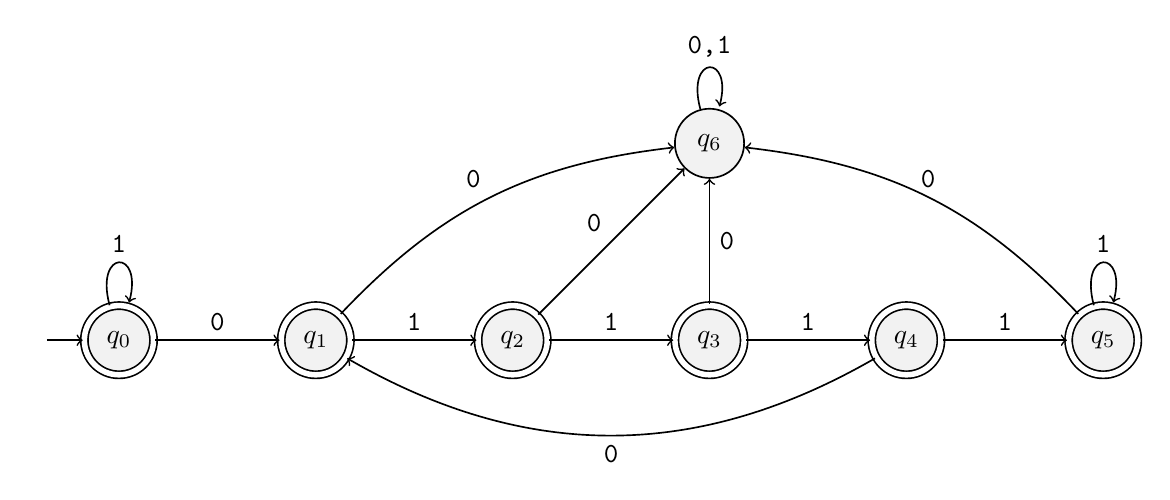
\begin{tikzpicture}
			\node[state, accepting, initial] (q0) {$q_0$};
			\node[state, accepting, right of=q0] (q1) {$q_1$};
			\node[state, accepting, right of=q1] (q2) {$q_2$};
			\node[state, accepting, right of=q2] (q3) {$q_3$};
			\node[state, accepting, right of=q3] (q4) {$q_4$};
			\node[state, accepting, right of=q4] (q5) {$q_5$};
			\node[state, above of=q3] (q6) {$q_6$};
			\draw (q0) edge[loop above] node {\tt 1} (q0);
			\draw (q5) edge[loop above] node {\tt 1} (q5);
			\draw (q6) edge[loop above] node {\tt 0,1} (q6);
			\draw (q0) edge node {\tt 0} (q1);
			\draw (q1) edge node {\tt 1} (q2);
			\draw (q2) edge node {\tt 1} (q3);
			\draw (q3) edge node {\tt 1} (q4);
			\draw (q4) edge node {\tt 1} (q5);
			\draw (q5) edge[bend right = 20] node [above] {\tt 0} (q6);
			\draw (q1) edge[bend left = 20] node {\tt 0} (q6);
			\draw (q2) edge node {\tt 0} (q6);
			\draw (q3) edge node [right] {\tt 0} (q6);
			\draw (q4) edge[bend left] node {\tt 0} (q1);
		\end{tikzpicture}	
\end{center}
	
	\begin{center}
			\begin{tabularx}{\textwidth}{|c|X|}
			\hline
			$q_0$ &		
			همه رشته‌های عضو 
			$\tt 1^*$
			در این حالت قرار دارند.
			\\ \hline
			$q_1$ &								
	رشته به صفر ختم شده است و تاکنون بین هر دو صفر که پشت هم ظاهر شده‌اند دقیقا ۳ یک قرار دارد.
			\\ \hline
			$q_2$ &						
			رشته به 
			$\tt 01 $ 
			ختم شده است و تاکنون بین هر دو صفر که پشت هم ظاهر شده‌اند دقیقا ۳ یک قرار دارد.
			\\ \hline
			$q_3$ &				
			رشته به 
			$\tt 011 $
			 ختم شده است و تاکنون بین هر دو صفر که پشت هم ظاهر شده‌اند دقیقا ۳ یک قرار دارد.
			\\ \hline
			$q_4$ &				
		رشته به 
		$ \tt 0111 $ 
		ختم شده است و تاکنون بین هر دو صفر که پشت هم ظاهر شده‌اند دقیقا ۳ یک قرار دارد.
			\\ \hline
			$q_5$ &
			رشته به حداقل ۴ یک ختم شده است و تاکنون بین هر دو صفر که پشت هم ظاهر شده‌اند دقیقا ۳ یک قرار دارد.
			\\ \hline
			$q_6$ &
			رشته شامل دو صفر پشت سر هم هست که بین آنها دقیقا ۳ یک قرار ندارد.
			\\ \hline
		\end{tabularx}
	\end{center}
	
		\item 
		
		\textcolor{cyan}{
			(9 نمره)
		}
	
\begin{minipage}{0.5\textwidth}
	\begin{tabularx}{\linewidth}{|c|X|}
		\hline
		$q_0$ &		
		رشته زوج صفر دارد و اگر 
		$\Lambda$
		نباشد به حداقل ۲ یک ختم شده است.
		\\ \hline
		$q_1$ &								
		رشته به صفر ختم شده است و فرد صفر دارد.
		\\ \hline
		$q_2$ &						
		رشته به 
		$\tt 01 $ 
		ختم شده است و فرد صفر دارد.
		\\ \hline
		$q_6$ &				
		رشته شامل 
		$\tt 010 $ 
		است.
		\\ \hline
		$q_3$ &				
		رشته به 
		$\tt 01 $
		ختم شده است و زوج صفر دارد.
		\\ \hline
		$q_4$ &
		رشته به صفر ختم شده است و زوج صفر دارد.
		\\ \hline
		$q_5$ &
		رشته فرد صفر دارد و به حداقل ۲ یک ختم شده است.
		\\ \hline
	\end{tabularx}	
\end{minipage}		
\begin{minipage}{0.5\textwidth}
			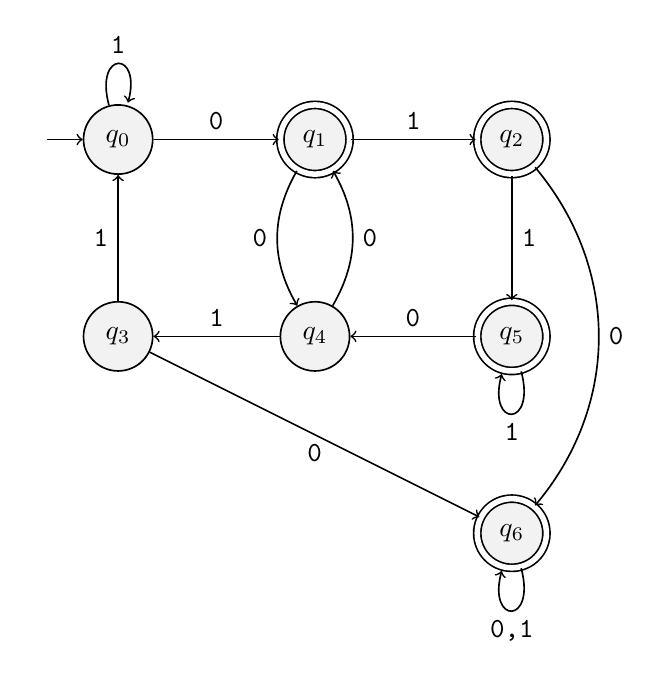
\begin{tikzpicture}
	\node[state, initial] (q0) {$q_0$};
	\node[state, accepting, right of = q0] (q1) {$q_1$};
	\node[state, accepting, right of = q1] (q2) {$q_2$};
	\node[state, below of =q0] (q3) {$q_3$};
	\node[state, below of = q1] (q4) {$q_4$};
	\node[state, accepting, below of = q2] (q5) {$q_5$};
	\node[state, accepting, below of = q5] (q6) {$q_6$};
	
	\draw (q0) edge[loop above] node {\tt 1} (q0);
	\draw (q0) edge node {\tt 0} (q1);
	
	\draw (q1) edge[bend right] node [left] {\tt 0} (q4);
	\draw (q1) edge node [above] {\tt 1} (q2);
	
	\draw (q2) edge[bend left = 40] node {\tt 0} (q6);
	\draw (q2) edge node {\tt 1} (q5);
	
	\draw (q3) edge node {\tt 1} (q0);
	\draw (q3) edge node [below] {\tt 0} (q6);
	
	\draw (q4) edge node [above]{\tt 1} (q3);
	\draw (q4) edge[bend right] node [right]{\tt 0} (q1);
	
	\draw (q5) edge node [above] {\tt 0} (q4);
	\draw (q5) edge[loop below] node  {\tt 1} (q5);
	
	\draw (q6) edge [loop below] node {\tt 0,1} (q6);
	
\end{tikzpicture}
\end{minipage}

	\end{enumerate}
\end{document}